\documentclass[a4paper,11pt]{article}
\usepackage[top=2cm,bottom=2cm,left=2cm,right=2cm]{geometry}
\usepackage[T1]{fontenc}
\usepackage[utf8]{inputenc}
\usepackage{lmodern}
\usepackage{textgreek}
\usepackage{amsmath}
\usepackage{mathtools}
\usepackage{graphicx}
\usepackage{svg}
\usepackage{pdflscape}

\usepackage{tabularx}
\usepackage{blindtext}
\usepackage{hyperref}
\usepackage{pgfgantt}
\usepackage{colortbl}
\usepackage{pdfpages}
\usepackage{setspace}


\setcounter{tocdepth}{3}
\begin{document}
	\begin{titlepage}
		\newcommand{\HRule}{\rule{\linewidth}{0.5mm}}
		\center
		\textsc{\Large University College London}\\[0.5cm]
		\textsc{\large Department of Electronic \& Electrical Engineering}\\[0.5cm]
		
		\HRule \\[0.4cm]
		\setstretch{1.5}
		{ \huge \bfseries Title}\\[0.4cm]
		\setstretch{1.0}
		\HRule \\[1.0cm]
		
		\Large \emph{Author:}\\
		Minduagas \textsc{Jarmolovi\v{c}ius}\\
		\href{mailto:zceemja@ucl.ac.uk}{zceemja@ucl.ac.uk}\\[0.5cm]
		
		\vfill
		\setstretch{2.5}
		{ \large \bfseries ELEC0134}\\[1cm]
		\setstretch{1.0}
		{\large\today}\\[2cm]
		
	\end{titlepage}
	
	\pagebreak
	
\section*{Abstract}
\iffalse
This section provides a brief overview of the methodology/results
presented in the report.
\fi

\section{Introduction}
\iffalse
This section introduces the problem, a brief bird’s-eye view
of the methodologies you adopted and the organization of this
report.
\fi


\section{Literature Survey}
\iffalse
This section should focus on an overview of potential ap-
proaches to solve the tasks. You can introduce some classical
and state-of-the-art machine learning algorithms.
\fi


\section{Description Of Models}
\iffalse
In this section, you should briefly describe the model you are
using for each task, along with the rationale. You may opt to
use a single learning algorithm to solve the problem or multi-
ple ones, but bear in mind there are page limitations and that
you should explain your rationale behind your choices. That
is, the algorithmic description must detail your reasons for
selecting a particular model.
You can clarify them with flow charts, figures or equa-
tions.
\fi


\subsection{Task A1: Gender classification}
\subsection{Task A2: Smile classification}
\subsection{Task B1: Face shape classification}
\subsection{Task B2: Eye colour classification}
\section{Implementation}
\iffalse
This section must provide the detailed implementation of your
models. In particular, you must provide the name and use of
external libraries, explain hyper-parameter selection, training
pipeline (if any) and key modules/classes/functions/algorithms.
You also must provide a detailed description of the dataset
(content, size, format, etc.), any data pre-processing that was
applied and how you separate your dataset into training, vali-
dation and test sets.
The execution of your models also should be reported
here. In particular, this section should include a thorough dis-
cussion on the training convergence and stopping criterion (it
is recommended that learning curves graphs be used to this
effect).
\fi

\subsection{Task A1: Gender classification}
\subsection{Task A2: Smile classification}

The first approach was to use face extraction method to detect lips (19 features with indices from 49 to 68 shown in \autoref{fig:face_features}) and try to train model only on these points. 
\begin{figure}[h]
	\centering
	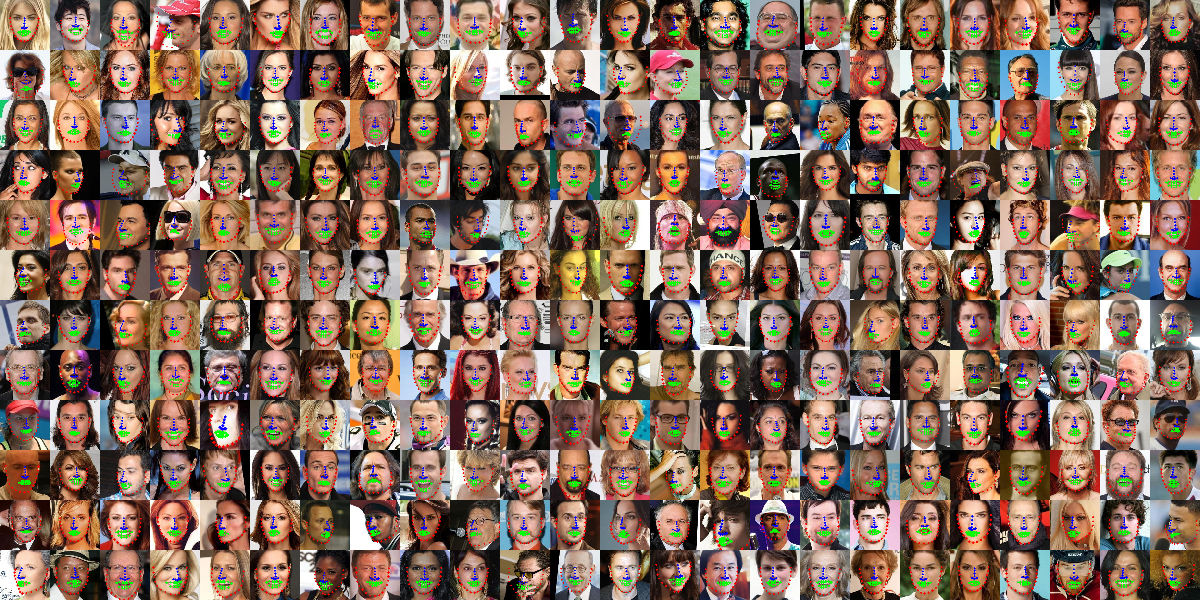
\includegraphics[width=\linewidth]{face_features2.png}
	\caption{Extracted face features for celebrity dataset, green for lips (indices 49-68), red for face shape (indices 1-17), blue for noise (indices 28-36)}
	\label{fig:face_features}	
\end{figure}
SVC model with 6th degree poly kernel, regularization parameter C of 0.07 yielded accuracy of 86.25\%. From \autoref{fig:face_features} it is visible that some lips are not classified correclty as model may detect chin instead. Also smile could be extracted from other features than a shape of a smile (e.g. cheeks and lip corners). As many pictures are quite noisy (e.g. there is an object in a front of mouth) these other face features might be essential to improve model accuracy. Cropping image around mouth within points 4, 9, 14, 31 and reducing gray image to 40 by 40 pixels with SVC 4th degree poly kernel with value C of 0.02 yielded worse accuracy of 85.27\%.

\subsection{Task B1: Face shape classification}
\subsection{Task B2: Eye colour classification}
\section{Experimental Results and Analysis}
\iffalse
This section describes and discusses your results. Addition-
ally, this section should include accuracy prediction scores on
a separate test dataset, provided by the module organizers, but
not used during your training and validation process.
We recommend you use a table to list the tasks, models
and results before analysis.
\fi

\iffalse
A1:
Model SVC(C=0.1, kernel='linear') scored 0.82004 (+/- 0.02509)
Model SVC(C=1, kernel='linear') scored 0.80486 (+/- 0.04161)
Model SVC(C=10, kernel='linear') scored 0.80154 (+/- 0.03218)
Model SVC(C=0.1) scored 0.78553 (+/- 0.04053)
Model SVC(C=1) scored 0.87056 (+/- 0.03118)
Model SVC(C=10) scored 0.88132 (+/- 0.02419)
Model SVC(C=0.1, kernel='poly') scored 0.63538 (+/- 0.03010)
Model SVC(C=1, kernel='poly') scored 0.84820 (+/- 0.02973)
Model SVC(C=10, kernel='poly') scored 0.86614 (+/- 0.04160)
Model SVC(degree=6, kernel='poly') scored 0.56528 (+/- 0.02749)
Model SVC(degree=9, kernel='poly') scored 0.52829 (+/- 0.02113)
Model RandomForestClassifier(n_jobs=-1) scored 0.72896 (+/- 0.05724)
Model RandomForestClassifier(n_estimators=200, n_jobs=-1) scored 0.75793 (+/- 0.03330)
Model RandomForestClassifier(n_estimators=300, n_jobs=-1) scored 0.75269 (+/- 0.04263)
Model RandomForestClassifier(n_estimators=400, n_jobs=-1) scored 0.75269 (+/- 0.04057)
Model RandomForestClassifier(n_estimators=500, n_jobs=-1) scored 0.75462 (+/- 0.04406)

Model SVC(C=0.1, kernel='linear') scored 0.99867 (+/- 0.00292)
Model SVC(C=1, kernel='linear') scored 0.99867 (+/- 0.00292)
Model SVC(C=10, kernel='linear') scored 0.99867 (+/- 0.00292)
Model SVC(C=0.1) scored 0.55440 (+/- 0.03589)
Model SVC(C=1) scored 0.90947 (+/- 0.02171)
Model SVC(C=10) scored 0.99133 (+/- 0.00708)
Model SVC(C=0.1, kernel='poly') scored 0.98813 (+/- 0.00839)
Model SVC(C=1, kernel='poly') scored 0.99773 (+/- 0.00317)
Model SVC(C=10, kernel='poly') scored 0.99893 (+/- 0.00232)
Model SVC(degree=6, kernel='poly') scored 0.99867 (+/- 0.00207)
Model SVC(degree=9, kernel='poly') scored 0.99747 (+/- 0.00437)
Model RandomForestClassifier(n_jobs=-1) scored 0.99840 (+/- 0.00373)
Model RandomForestClassifier(n_estimators=200, n_jobs=-1) scored 0.99880 (+/- 0.00303)
Model RandomForestClassifier(n_estimators=300, n_jobs=-1) scored 0.99880 (+/- 0.00278)

[2020-12-14 09:57:33,128][B1.train][INFO] Starting task B1 training ..
[2020-12-14 09:57:57,819][B2.__init__][INFO] Creating task preprocessing ..
Model SVC(C=0.1, kernel='linear') scored 0.99067 (+/- 0.01025)
Model SVC(C=1, kernel='linear') scored 0.99067 (+/- 0.01025)
Model SVC(C=10, kernel='linear') scored 0.99067 (+/- 0.01025)
Model SVC(C=0.1) scored 0.27069 (+/- 0.05624)
Model SVC(C=1) scored 0.89094 (+/- 0.03127)
Model SVC(C=10) scored 0.96193 (+/- 0.02160)
Model SVC(C=0.1, kernel='poly') scored 0.98158 (+/- 0.01225)
Model SVC(C=1, kernel='poly') scored 0.98526 (+/- 0.01076)
Model SVC(C=10, kernel='poly') scored 0.98526 (+/- 0.01076)
Model SVC(degree=6, kernel='poly') scored 0.96856 (+/- 0.01530)
Model SVC(degree=9, kernel='poly') scored 0.94793 (+/- 0.01969)
Model RandomForestClassifier(n_jobs=-1) scored 0.98797 (+/- 0.01149)
Model RandomForestClassifier(n_estimators=200, n_jobs=-1) scored 0.98895 (+/- 0.00912)
Model RandomForestClassifier(n_estimators=300, n_jobs=-1) scored 0.98969 (+/- 0.00975)
Model RandomForestClassifier(n_estimators=400, n_jobs=-1) scored 0.98895 (+/- 0.00884)
Model RandomForestClassifier(n_estimators=500, n_jobs=-1) scored 0.99091 (+/- 0.01007)
[2020-12-14 10:36:18,594][B2.test][INFO] Task B2 model achieved 99.5\% accuracy
\fi

















\begin{table}[h!]
	\begin{center}
		\begin{tabular}{l|c|c|c|c} 
			& \textbf{Task A1} & \textbf{Task A2} & \textbf{Task B1} & \textbf{Task B2}\\
			\hline
SVC Linear C=0.1    & 0.82004 & - & 0.99867 & 0.99067 \\
SVC Linear C=1      & 0.80486 & - & 0.99867 & 0.99067 \\
SVC Linear C=10     & 0.80154 & - & 0.99867 & 0.99067 \\
SVC RBF C=0.1       & 0.78553 & - & 0.55440 & 0.27069 \\
SVC RBF C=1         & 0.87056 & - & 0.90947 & 0.89094 \\
SVC RBF C=10        & 0.88132 & - & 0.99133 & 0.96193 \\
SVC Poly C=0.1 D=3  & 0.63538 & - & 0.98813 & 0.98158 \\
SVC Poly C=1 D=3    & 0.84820 & - & 0.99773 & 0.98526 \\
SVC Poly C=10 D=3   & 0.86614 & - & 0.99893 & 0.98526 \\
SVC Poly C=1 D=6    & 0.56528 & - & 0.99867 & 0.96856 \\
SVC Poly C=1 D=9    & 0.52829 & - & 0.99747 & 0.94793 \\
Random Forest N=100 & 0.72896 & - & 0.99840 & 0.98797 \\
Random Forest N=200 & 0.75793 & - & 0.99880 & 0.98895 \\
Random Forest N=300 & 0.75269 & - & 0.99880 & 0.98969 \\
Random Forest N=400 & 0.75269 & - & - & 0.98895  \\
Random Forest N=500 & 0.75462 & - & - & 0.99091  \\
		\end{tabular}
		\caption{Accuracy of different models}
		\label{tab:table1}
	\end{center}
\end{table}


\section{Conclusion}
\iffalse
This last section summarizes the findings and suggests direc-
ions for future improvement.
\fi


\section{References}

\end{document}